\section{Voxel data surface reconstruction}
\label{sec:surfaceBackg}
\todo[inline]{Benni: Don't overuse acronyms}
In order to fit \ac{NURBS} and other curves to an optimized geometry, a \emph{mesh-based geometry}, that is, a representation of the object at a set of (connected) points, is typically needed, this as opposed to the volumetric representation of density in each voxel, that results from the topology optimization process. 

In order to produce the mesh-based geometry, the data can be represented by a contour at a value of a smooth function in space, that is, an isosurface. Below, we describe four methods that solve this problem, the \acl{MC}, the \acl{DC}, the \acl{DualMC} and the \acl{DualMT} method. This section is only intended for giving a brief overview over the different methods and the most important properties regarding our application. For more details we refer to \cite{Marching2006, Hermite2002, Nielson2004, Nielson2008}. 

\todo[inline]{Benni: this remark is useful. But explain in more detail. Change sentence, explain what in particular voxel surface reconstruction is. Leave out range surface reconstruction.} One should also note that surface reconstruction from voxel data --- what we are doing --- and surface reconstruction from range scan data (for example see \todo{give example}) are similar, but still different tasks.

% subsection on Marching Cubes
\subsection{\Acl{MC}} 
\tododone[inline]{Proofreading of Benni \& JC}
The \acf{MC} method \cite{Marching2006} takes as an input a set of scalar function values on a Cartesian mesh and extracts an approximate isosurface in the form of a mesh of triangles. The method starts by dividing the space into cubes with the set of function values as cube vertices. These values are determined to be above or below the desired isovalue. According to which corners are set to be above or below, the corner configuration is then mapped to a polygon inside the cube, with vertices on the cube's edges. On an edge between a vertex above and a vertex below the desired isovalue, the exact location of the surface is determined via linear interpolation. Then this location is set as the polygon's vertex on that edge. A result of the \ac{MC} algorithm is shown in \autoref{fig:bunny}.

\begin{figure}
\centering
   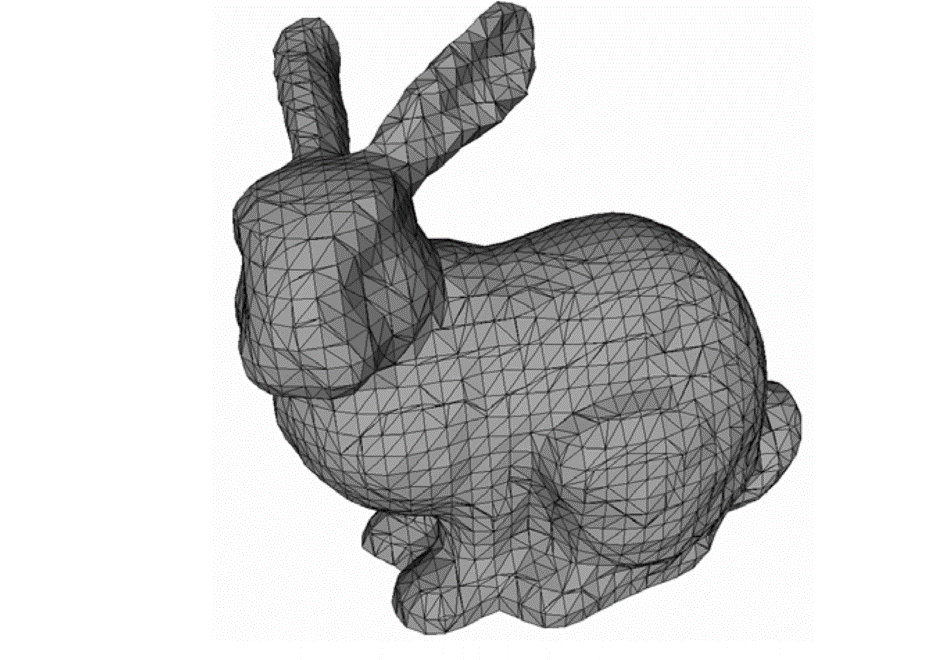
\includegraphics[width=.25\textwidth]{Pictures/SurfaceReconstruction/new_bunny.png}
   \caption{The famous Stanford Bunny, a popular computer graphics test object, here after application of \ac{MC}. Figure from \cite{NielsonParametrization}. }
   \label{fig:bunny}
\end{figure}


\subsubsection{The \acl{MC} cases}
Since there are 8 vertices on each cube, either above or below the isovalue (with equality falling to one of these categories), $2^8=256$ possible polygon configurations exist. However, many of these can be constructed by rotating or reflecting other polygons. Therefore 15 base cases which represent all the surface polygons of the \acl{MC} are sufficient to take into consideration. \autoref{fig:MC_basecase} shows how these base cases look like, we can notice that they are composed of triangles. 

\begin{figure}
\centering
   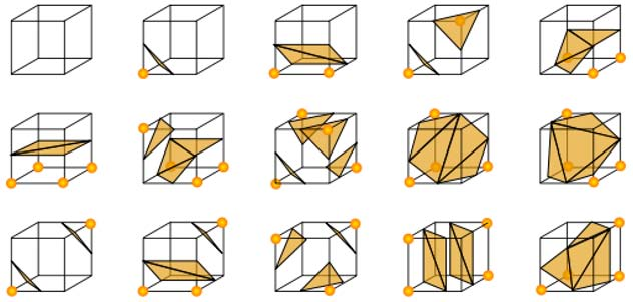
\includegraphics[width=.5\textwidth]{Pictures/cubes.pdf}
   \caption{The base cases of \ac{MC}. These are drawn with each polygon vertex intercepting its edge in the middle between the cube's corners, as in the case when the isovalue is exactly halfway between the function values at the vertices. Figure from \cite{Marching2006}.}
   \label{fig:MC_basecase}
\end{figure}

\subsubsection{Cracks and ambiguities}
The original algorithm presents two main problems. Firstly, it guarantees neither correctness nor topological consistency, which means that holes may appear on the surface due to inaccurate base case selection. The second problem is ambiguity, which appears when two base cases are possible and the algorithm chooses the incorrect one, or cannot decide on one. There are many extended \ac{MC} algorithms that tackle the problems of the original one, getting rid of the ambiguities and providing correctness (see for example \cite{ExtendedMC}).


% subsection on Dual Contouring
\subsection{\Acl{DC}}
\tododone[inline]{Proofreading of Benni \& JC}
\todointern[inline]{generally longer, more explanatory captions}
\label{ssec:DC}
The idea of \emph{dual algorithms}, to which \acf{DC} belongs, is similar to \ac{MC}. However, instead of generating polygon vertices on the edges of the cubes, this method locates them inside the cubes that have at least one edge which has vertex values both above and below the isovalue (\acs{SignChangingEdge}). The basic algorithm can be summarized in these two steps:
\begin{enumerate}
\item Locate the position of the vertex inside each cube which has at least one \ac{SignChangingEdge}.
\item Join the vertices associated with four cubes sharing a common edge to form a \ac{quad}.
\end{enumerate}
The approach can be seen in \autoref{fig:bunny_MCDC}, with a similar \ac{MC} illustration for comparison.

\begin{figure}
\centering
   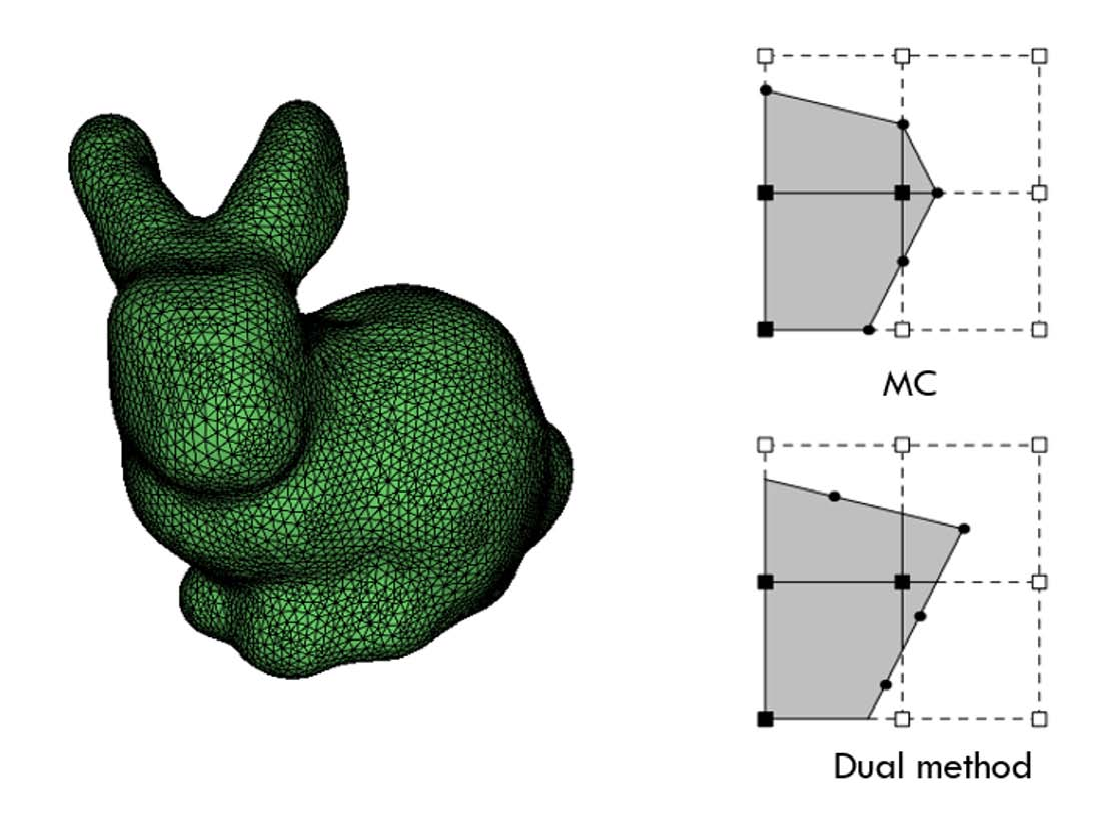
\includegraphics[width=.5\textwidth]{Pictures/bunny_MC.pdf}
   \caption{\textit{Left:} The famous Stanford Bunny, a popular computer graphics test object, here after application of \ac{MC}. \textit{Right:} Main difference between \ac{MC} and \ac{DC}.  Figures taken from \cite{Hermite2002}. }
   \label{fig:bunny_MCDC}
\end{figure}

\subsubsection{Minimizing the \acl{QEF}}
Now we want to find out where in the cube the ideal place for the vertex is located, and here different dual algorithms are distinguished. \Ac{DC} in particular generates a vertex positioned at the minimizer of a certain quadratic function. This function depends on the (interpolated) isosurface intersection points, as well as the gradient -- or just the normal of the isosurface -- at these points, both quantities represent the \acs{FirstOrderHermiteData} of the set.
The \acl{QEF} is defined in \cite{Hermite2002} as follows:
\begin{equation}
\label{eq:QEF}
E(x)= x^TA^TAx-2x^TA^Tb+b^Tb
\end{equation}
where the columns of the matrix \textit{A} are the  isosurface normals at the intersection points, and \textit{b} is a vector containing the scalar product of the normals and the intersection points. This system can be solved numerically, for example as proposed in \cite{Hermite2002} by computing the singular value decomposition of \textit{A} and forming the pseudo-inverse, truncating its small singular values. 
The effect of considering the gradient for the calculation of the vertex is huge: \ac{DC} has the ability to represent sharp features like edges and corners.
Computing the position of the new node by just taking the mean value of all the roots on the \acsp{SignChangingEdge} of one cube represent an easier approach, which does not rely on gradient information, but is also not able to represent sharp features. The resulting vertex is inside the cube, because it represents the average position of the nodes lying on edges of the cube.

\subsubsection{Non-manifold surfaces}
The risk to also obtain non-manifold surfaces represents one of the big drawbacks of \ac{DC}. A manifold surface is defined by the following topological property:
\begin{quote}
\emph{A $d$-dimensional contour is locally a \emph{manifold} if it is topologically equivalent to a $d$-dimensional disc.}\cite{Hermite2002}
\end{quote}
This means that for 2D data we only get a manifold isocontour, if each vertex is connected to exactly 2 edges. For 3D we only get a manifold isosurface, if each edge is at maximum shared by two \acp{quad}. Since the original method does not deal with this issue, extensions have been developed to solve this problem.\autoref{fig:manifold}) shows one configuration creating a non-manifold surface for the basic method from \cite{Hermite2002} and its correct resolution by \cite{Schaefer2007}.
\todo[inline]{\ref{fig:manifold} put all subfigures into one line}

\begin{figure}
\begin{center}
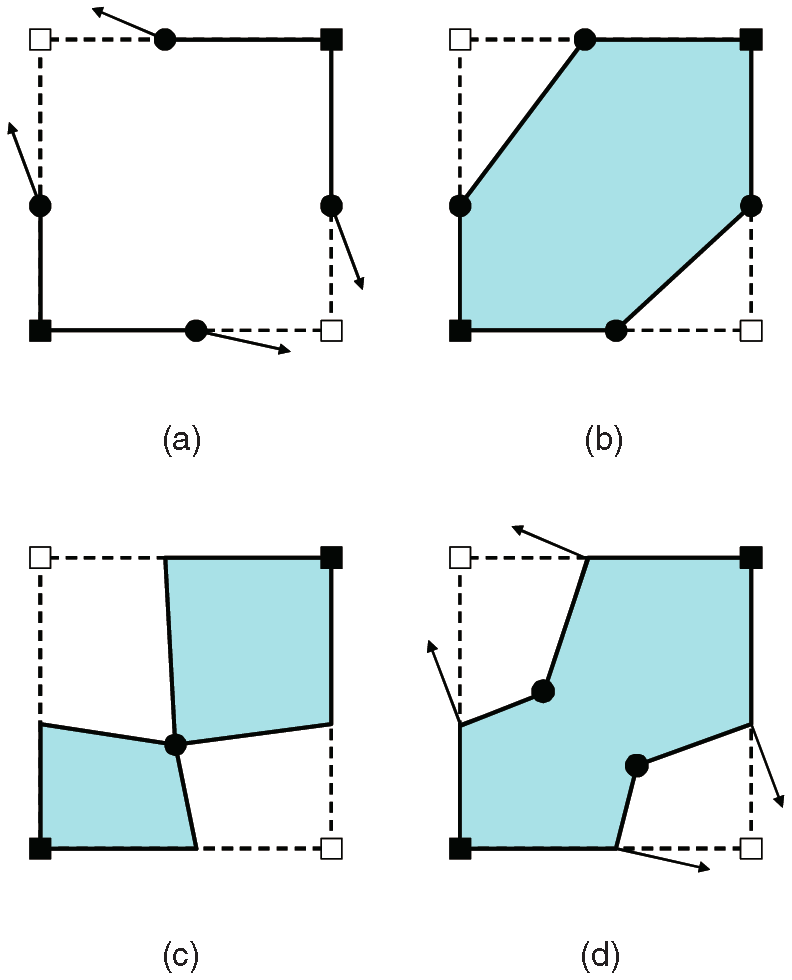
\includegraphics[width=.3 \textwidth]{Pictures/SurfaceReconstruction/ManifoldDC.png}
\end{center}
\label{fig:manifold}
\caption{Comparison of contouring for Hermite data. (a) Cell with Hermite data on edges, (b) manifold contour from \acs{MC}, (c) non-manifold contour from \acs{DC}, (d) manifold contour from \acs{DualMC} (figure and description from \cite{Schaefer2007})}
\end{figure}

\subsubsection{Topology-safe adaptivity}
Usually having as few faces as possible is desirable for reasons like filesize and complexity of the mesh. But in its basic form \ac{DC} is working with uniformly distributed data and introduces vertices on a uniform grid. The reconstructed surface mesh has uniform resolution on the whole area and this results in huge files and a uniformly high resolution, if one wants to resolve fine features of the geometry. As a post processing step one could try to simplify the mesh, but especially for \ac{quad} meshes this is a very demanding -- sometimes even impossible -- task \cite{Puppo2010}.

The solution to this problem is adaptivity. Referring to \cite{Hermite2002} it is possible to implement \ac{DC} in an adaptive and topology-safe way. This means we can simplify the obtained \ac{quad} mesh and therefore reduce the number of \acp{quad} needed to represent the surface, while still conserving the topological structure of our surface.


% subsection on Dual Marching Cubes
\subsection{Dual Marching Methods}
\todo[inline]{Benni: this part is more a outlook than something which has been implemented, remove this and keep it for next milestone? If yes, don't forget to remove the references in the introduction of this chapter!}
So far we have introduces \ac{MC} and \ac{DC} and discovered that both methods have certain drawbacks:
\begin{itemize}
\item \ac{MC} always produces manifold surfaces and resolves ambiguities correctly, while \ac{DC} does not have this property.
\item \ac{DC} has the ability to produce \ac{quad} surfaces and preserve sharp features, while \ac{MC} produces surfaces consisting of \acp{tri}\footnote{The construction of \acp{tri} is not a drawback of the \ac{MC} method in general, but for our purpose we have to construct \acp{quad} and therefore this point is crucial. If we want to finally produce a \ac{NURBS} surface, we have to rely on \acp{quad}, because \ac{NURBS} have a rectangular topology. \Acp{tri} just do not fit the topology of \ac{NURBS}. Further explanation can be found in \autoref{sec:NURBS} and \autoref{sec:surfaceImpl}} and sharp features are often lost.
\end{itemize}
To come up with these drawback, hybrid methods have been developed. These methods use ideas from both the \ac{MC} and the \ac{DC} world (For a short summary of those ideas see \autoref{tab:dualmarching}).
\tododone[inline]{Benni: Change table}
\begin{table}[H]
\begin{tabularx}{\textwidth}{X|X}
\multicolumn{1}{c|}{\acl{MC}} 
    & \multicolumn{1}{c}{\acl{DC}} 
\\
\hline
\begin{itemize}[noitemsep, topsep = 0pt, leftmargin=1em]
\item traverse voxels and use a look up table for the creation of faces
\item creates manifold and ambiguity free surfaces
\end{itemize}
&
\begin{itemize}[noitemsep, topsep = 0pt, leftmargin=1em]
\item place vertices inside voxel\footnote{Determine positions by -- for example -- minimizing \autoref{eq:QEF}.}
\item construct \acp{quad} by joining vertices in voxels with a common edge
\end{itemize}
\end{tabularx}
\caption{ideas from \ac{DC} and \ac{MC} contributing to dual marching methods.}
\label{tab:dualmarching}
\end{table}

\subsubsection{\acl{DualMC}}
The \acf{DualMC} method is --- like already stated above --- a hybrid of \ac{MC} and \ac{DC}: We traverse the cubes like in \ac{MC} and insert vertices and connect them like in \ac{DC}. The combination of the $256$ different cases from the basic \ac{MC}, the extension for creating ambiguity free surfaces and the framework of \ac{DC} results in a very effective but also complex algorithm. A drawback of this method is that for certain configurations we have to create non-\ac{quad} faces --- especially faces with odd number of vertices are difficult to convert to \acp{quad}, if one wants to obtain a \ac{quad}-only surface like in \ac{DC}. We refer the interested reader to  \cite{Nielson2004, Zhang2012}.

\begin{figure}
\begin{center}
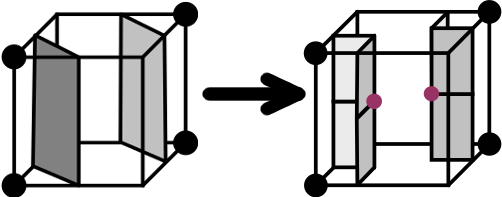
\includegraphics[width = .5\textwidth]{Pictures/SurfaceReconstruction/MCtoDualMC.png}
\end{center}
\caption{How one of the \ac{MC} cases is treaten in \ac{DualMC} algorithm (figure from \cite{Nielson2004})}
\end{figure}

\subsubsection{\acl{DualMT}}
While \ac{DualMC} is a very complicated algorithm, \acf{DualMT} uses tetrahedra instead of cubes and therefore reduces the $256$\footnote{With a proper treatment of ambiguities we get even more than those $256$ cases.} different cases from \ac{MC} to $2^4=16$ cases. Furthermore a treatment of ambiguous cases is not necessary anymore, since there are no ambiguous cases for this method\todo{really? check this or find reference!}.
Even though the method is working on tetrahedra, we can still apply it to a voxel dataset, by composing each cube out of 5 or 6 tetrahedra (\autoref{fig:splittingCubes}). But this high amount of simplifictaion comes with a drawback: The treatment of ambiguous cases depends on the splitting scheme applied to a cube\todo{proof or reference! Show 2D example.}. Further detail on this method can be found in \cite{Nielson2008}.

\begin{figure}
\begin{center}
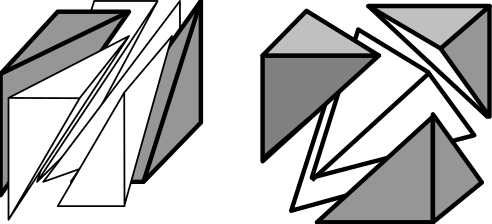
\includegraphics[width = .5 \textwidth]{Pictures/SurfaceReconstruction/SplittingCubes.png}
\caption{Two different subdivision schemes for cubes into tetrahedra (figure from \cite{Nielson2008})}
\label{fig:splittingCubes}
\end{center}
\end{figure}